\chapter{Automatic Street Light}

Switching street lights ON and OFF at different times of the day is a real hassle and an inefficiency in its control leads to waste of electricity. In this project, we will automate the switching of a light according to the brightness level in its surroundings. Instead of an actual street light, we will be using an LED for this project.

\subsection*{Components}
\begin{table}[H]
    \centering
    \begin{tabular}{|c|l|c|}\hline
     \textbf{\#} & \textbf{Components}  & \textbf{Amount}\\\hline
     1 & LEDs                               & 3\\\hline
     2 & 470 $\Omega$ resistor              & 3\\\hline
     3 & LDR     & 3 \\\hline
     4 & 10 k$\Omega$ resistor              & 3\\\hline
     5 & Arduino UNO                        & 1 \\\hline
     6 & Connecting Wires                   & - \\\hline
    \end{tabular}
\end{table}

\subsection*{Connections}

\begin{enumerate}[leftmargin=*]
    \item Connect 470 $\Omega$ resistor with the anode of all LEDs. 
    \item Connect each of the other end of the resistors to pins 4, 5, and 6 of Arduino separately.
    \item Connect the cathode of all LEDs to GND of Arduino
    \item Connect 10 k$\Omega$ resistors with one end of all LDRs. 
    \item Connect the other end of the resistors to GND of Arduino. 
    \item Connect the free end of all LDRs to 5V of Arduino.
    \item Connect the junctions of the LDRs and resistors to pins A0, A1, and A2 of Arduino respectively. 

\end{enumerate}
Fig. \ref{fig:street} illustrates the connections.

	\begin{figure}[!ht]
	\centering 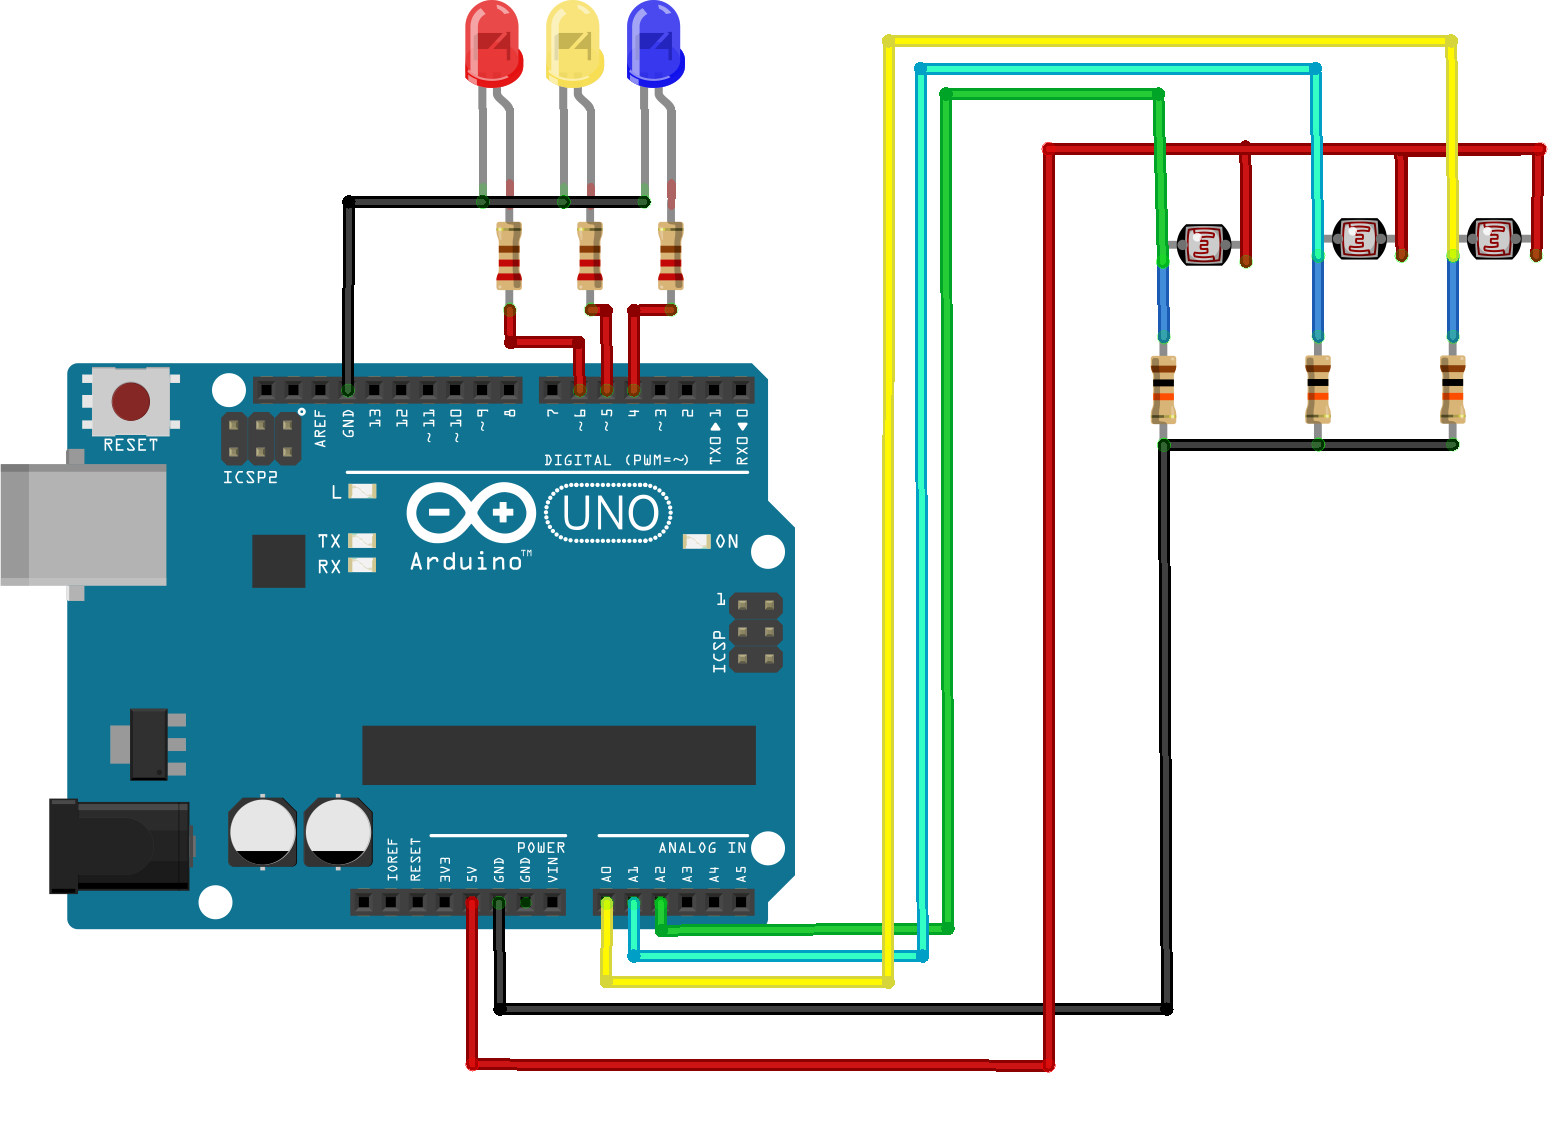
\includegraphics[width=0.6\linewidth]{Figures/recreational_exp/led with LDR_bb.png}
	\caption{Circuit diagram of LED controlled with LDR}
	\label{fig:street}
	\end{figure}
	
\subsection*{Procedure}
\begin{enumerate}[leftmargin=*]
     \item Copy lst. \ref{list:led-with-ldr} to a new Arduino sketchbook. Upload the code to your Arduino board. 
    \item Open flashlight of your mobile and shine it on one of the LDRs and see the change in state of cthe orresponding LED. 
    \item Repeat this process with other LDRs. 
\end{enumerate}
	
\begin{lstlisting}[language=Arduino, numbers=none, caption={Code for bluetooth-controlled car}, captionpos=b, label={list:led-with-ldr}]
// LED pins
int LED1 = 4;
int LED2 = 5;
int LED3 = 6;


//LDR pins
int LDR1 = A0;
int LDR2 = A1;
int LDR3 = A2;

//variables to save LDR values 
int in1, in2, in3;

int threshhold = 200; //set value according to your environment

void setup() {
  // put your setup code here, to run once:
pinMode(LED1, OUTPUT);
pinMode(LED2, OUTPUT);
pinMode(LED3, OUTPUT);
pinMode(LDR1, INPUT);
pinMode(LDR2, INPUT);
pinMode(LDR3, INPUT);
}

void loop() {
    // put your main code here, to run repeatedly:

    in1 = analogRead(LDR1);
    in2 = analogRead(LDR2);
    in3 = analogRead(LDR3);

    //LED1
    if (in1>threshhold)
        digitalWrite(LED1, HIGH);
    else
        digitalWrite(LED1, LOW);

    //LED2
    if (in2>threshhold)
        digitalWrite(LED2, HIGH);
    else
        digitalWrite(LED2, LOW);

    //LED3
    if (in3>threshhold)
        digitalWrite(LED3, HIGH);
    else
        digitalWrite(LED3, LOW);
}
\end{lstlisting}